\documentclass[11pt,a4paper]{article}

\usepackage{graphicx}
\usepackage{xcolor}
\usepackage[left=2.5cm, right=2.5cm, top=2.5cm, bottom=2.5cm]{geometry}
\usepackage{amsmath,amssymb,amsthm}
\usepackage{fontspec}
\setmainfont{Liberation Serif}
\setsansfont{Liberation Sans}
\setmonofont{Liberation Mono}[Scale=0.86]
\usepackage[russian]{babel}
\usepackage{booktabs}
\usepackage{tabularx}
\newcolumntype{Y}{>{\raggedright\arraybackslash}X}
\usepackage{colortbl}
\usepackage{adjustbox}
\usepackage{enumitem}
\usepackage{tcolorbox}
\usepackage[
    colorlinks=true,
    linkcolor=linkblue,
    citecolor=darkgray,
    urlcolor=linkblue,
    bookmarks=true,
    bookmarksnumbered=true,
    unicode=true
]{hyperref}

\definecolor{linkblue}{HTML}{1e3a5f}
\definecolor{accgreen}{HTML}{0e7c66}
\definecolor{warnamber}{HTML}{b45309}
\definecolor{rowlight}{HTML}{f0f5fa}

\widowpenalty=10000
\clubpenalty=10000
\emergencystretch=1.8em
\tolerance=2500

\theoremstyle{plain}
\newtheorem{theorem}{Теорема}[section]
\newtheorem{lemma}[theorem]{Лемма}
\newtheorem{proposition}[theorem]{Предложение}
\newtheorem{corollary}[theorem]{Следствие}
\theoremstyle{definition}
\newtheorem{definition}[theorem]{Определение}
\theoremstyle{remark}
\newtheorem{remark}[theorem]{Замечание}

\renewcommand\proofname{Доказательство}

\newtcolorbox{honestybox}[1][]{colback=warnamber!6, colframe=warnamber!80,
  title={\textbf{Честность:} #1}, fonttitle=\small, boxrule=0.7pt, arc=2pt}
\newtcolorbox{lemmabox}[1][]{colback=rowlight, colframe=linkblue,
  title={#1}, fonttitle=\bfseries\small, boxrule=0.9pt, arc=2pt}

\setlist[itemize]{leftmargin=1.5em, itemsep=1pt, topsep=2pt}

\hypersetup{
    pdftitle={Лемма Ш.3: равномерная устойчивость кунцевского дефекта — острая теорема следа и мост (iii)},
    pdfauthor={wild8highlander / choptuik_ac_bc},
    pdfsubject={Отдельная статья: острая теорема следа F >= 5n/7 и развёртка шага Ш.3(iii)},
    pdfkeywords={sofic groups, Leavitt algebra, Kunze defect, uniform stability, sharp trace theorem, 5n/7}
}

\begin{document}

% Обложка генерируется отдельно (HTML/Playwright) и подшивается страницей 0.

\tableofcontents
\newpage

\begin{center}
{\Large\bfseries Аннотация}\par\medskip
\end{center}
\noindent
Настоящая статья выделяет из приложения «Аудит и перенос» шаг~Ш3 цепочки
переноса и разворачивает его в самостоятельный аналитический объект —
\emph{лемму Ш.3 о равномерной устойчивости кунцевского дефекта}. Центральный
результат — \emph{острая теорема следа}: для всех $n\ge 1$ и всех
$X_1,X_2\in M_n(\mathbb{C})$ кунцевский дефект
$F(X_1,X_2)\ge 5n/7$, причём равенство достигается в точности на парах
$X_1X_1^*=X_2X_2^*=(4/7)I$. Доказательство проводится полной редукцией:
тождество $F=G(P,Q)$ при $P=X_1X_1^*$, $Q=X_2X_2^*$, строгая выпуклость
$G$ и инвариантность относительно одновременного унитарного сопряжения
сводят задачу к усреднению по Хаару, а скалярный минимум даёт ровно
$5n/7$. Тем самым \emph{дефект на душу размерности зажан универсальной
константой $e\ge 5/7$ при всех масштабах} — «поправка, работающая в
бесконечность» получает точный аналитический смысл. Попутно исправлена
ошибка версии v1.0 приложения: утверждавшийся там пол $n/2$ опирался на
неверную минимизацию трёхчлена (фактический минимум $n/3$); острая
теорема заменяет эту цепочку и доказывает глобальный минимум $5n/7$,
который в v1.0 был только численной гипотезой. Часть~(iii) леммы —
\emph{мост}: если $G=U(L_{\mathbb{F}_2}(1,2))$ софична, то существуют
матричные модели с дефектом на душу $e_k\le\eta(\varepsilon_k)\to 0$,
где $\eta(\varepsilon)=C\,\varepsilon^{1/2}$ универсальна; вместе с
острой теоремой это даёт противоречие $5/7\le e_k\to 0$ и, условно
по~(iii), несофичность $G$. Перестановочные модели с точными первыми
соотношениями дают дефект $F=2n$ — софическая сторона не обходит пол, а
усиливает его. Вся численная часть реализована на Python и Julia,
детерминирована и воспроизводится одной командой каждая.

\section{Введение: место леммы в цепочке переноса Ш1--Ш4}\label{sec:intro}

Фреймворк Исаева--Чоптьюка переносит поправки, выведенные из первых
принципов для критического коллапса Чоптьюка (бэровская
$b\text{-}C=\delta_C^2/2$, тормозная $a\text{-}C=\delta_C^5/22$ и третья
$\mathcal C$), на задачи, в которых препятствие должно «работать в
бесконечность». Приложение «Аудит и перенос» изложило этот перенос в виде
цепочки из четырёх шагов Ш1--Ш4, где каждый шаг опирается на предыдущий и
проверяется машинно. Шаг~Ш3 был там сформулирован одним предложением:
«софическая аппроксимация группы единиц индуцировала бы матричные модели
кунцевских соотношений с убывающим дефектом» — с пометкой, что здесь
работает лемма равномерной устойчивости. Настоящая статья разворачивает
это предложение в явную формулировку, доказывает её матричную часть
\emph{в острой форме} и отдаёт всё под численный контроль.

Полная цепочка в замкнутом виде выглядит следующим образом. Шаг~Ш1:
класс $[1]=0$ в $K_0$-группе и острый дефект кунцевских соотношений
$5n/7$ на душу размерности в каждой полной матричной алгебре $M_n$ —
это теорема~\ref{th:sharp} настоящей статьи. Шаг~Ш2: никакая
последовательность матричных моделей не даёт дефекта на душу, стремящегося
к нулю, — прямое следствие теоремы~\ref{th:sharp}: константа $5/7$
универсальна и от масштаба не зависит. Шаг~Ш3: софичность группы единиц
индуцировала бы модели с дефектом на душу $\to 0$ — это содержание моста,
части~(iii). Шаг~Ш4: соединение Ш1--Ш3 даёт противоречие, значит
$G=U(L_{\mathbb{F}_2}(1,2))$ несофична — условное заключение,
замыкаемое частью~(iii).

Ключевая идея, которую статья фиксирует явно: поправки фреймворка
«работают в бесконечность» в том точном смысле, что \emph{дефект на душу
размерности зажат универсальной константой}, не зависящей от масштаба
$n$. Именно поэтому никакое увеличение матричных моделей не размывает
препятствие: у свободной группы $\mathbb{F}_2$ дефекты слов размываются
вдоль случайных перестановочных моделей (минимальный Хэмминг
$\ge 0.9$ и растёт с $N$), а у пары Ливитта пол на душу стоит на месте
при всех $n$. Это контраст механизмов «размывание против пола», и он
демонстрируется численно в разделе~\ref{sec:numeric}.

Отдельно зафиксируем редакторскую историю. Версия v1.0 приложения
утверждала пол $F\ge n/2$ «однострочным» доказательством через следовые
оценки; настоящая версия исправляет эту цепочку (замечание
~\ref{rem:v1}) и усиливает результат до острого $5n/7$ с полной
характеризацией равенства. Численные таблицы v1.0 при этом не меняются
по существу: минимизация и раньше выходила на $5n/7$ — изменился статус
этого числа, из численной гипотезы оно стало теоремой.

\section{Матричный кунцевский дефект: постановка}\label{sec:setup}

Фиксируем обозначения и объект. Все нормы ниже — нормы Фробениуса,
$I=I_n$ — единичная матрица порядка $n$, звезда $*$ — эрмитово
сопряжение. Кунцевские соотношения пары Ливитта
$L_{\mathbb{F}_2}(1,2)$ в матричной постановке — это система
\begin{equation}
x_1^*x_1 = 1,\qquad x_2^*x_2 = 1,\qquad x_1^*x_2 = 0,\qquad
x_1x_1^* + x_2x_2^* = 1.
\label{eq:kunze}
\end{equation}
«Моделью соотношений» в $M_n(\mathbb{C})$ называется любая пара
$(X_1,X_2)\in M_n(\mathbb{C})^2$; пара называется точным решением, когда
все четыре равенства выполнены знак в знак.

\begin{definition}[кунцевский дефект]\label{def:defect}
Для пары $(X_1,X_2)\in M_n(\mathbb{C})^2$ положим
\begin{equation}
F(X_1,X_2) \;=\; \|X_1^*X_1-I\|_F^2 + \|X_2^*X_2-I\|_F^2
+ \|X_1^*X_2\|_F^2 + \|X_1X_1^*+X_2X_2^*-I\|_F^2,
\label{eq:F}
\end{equation}
и назовём величину $e(X_1,X_2) = F(X_1,X_2)/n$ \emph{дефектом на душу
размерности}. Пара точна тогда и только тогда, когда $F=0$.
\end{definition}

\begin{definition}[софичность]\label{def:sofic}
Группа $G$ софична, если существуют $n_k\to\infty$ и отображения
$\rho_k\colon G\to\mathrm{Sym}(n_k)$ такие, что для некоторого конечного
порождающего $F_0\subseteq G$ и $\varepsilon_k\to 0$ выполнено:
(С1) $\mathrm{Hamming}(\rho_k(w),\mathrm{id})/n_k\ge 1-\varepsilon_k$
для всех $w\in F_0$, $w\ne e$; (С2) $\rho_k$ — приближённые
гомоморфизмы на словах длины $\le L(F_0)$ с ошибкой $\le\varepsilon_k$
(стандартное определение Громова).
\end{definition}

Функционал \eqref{eq:F} — это сумма четырёх квадратичных невязок,
по одной на каждое соотношение \eqref{eq:kunze}; он неотрицателен и
обращается в нуль только на точных решениях. Выбор нормы Фробениуса
существенен: именно она даёт и следовую структуру тождества
раздела~\ref{sec:sharp}, и точную характеризацию равенства. Дефект на
душу $e$ — правильный масштаб для вопроса об «устойчивости в
бесконечность»: если бы существовала последовательность моделей с
$e\to 0$, препятствие считалось бы размытым; теорема~\ref{th:sharp}
показывает, что это невозможно уже внутри одной $M_n$. Замечание о
точных решениях: в $M_n(\mathbb{C})$ точные решения системы
\eqref{eq:kunze} не существуют ни при каком $n\ge 1$: равенство
$X_1^*X_1=I$ делает $X_1$ унитарной, откуда $X_1X_1^*=I$ и четвёртое
соотношение даёт $X_2X_2^*=0$, то есть $X_2=0$ — в противоречии с
$X_2^*X_2=I$. Препятствие, таким образом, не в отсутствии решений в
отдельной алгебре, а в том, что дефект отделён от нуля \emph{равномерно
по $n$} — теорема~\ref{th:sharp}.

\section{Часть (i): острая теорема следа $F\ge 5n/7$}\label{sec:sharp}

\begin{theorem}[острая теорема следа]\label{th:sharp}
Для всех $n\ge 1$ и всех $X_1,X_2\in M_n(\mathbb{C})$
\[
F(X_1,X_2)\;\ge\;\frac{5n}{7},
\]
причём равенство достигается тогда и только тогда, когда
$X_1X_1^*=X_2X_2^*=\tfrac47 I$ (эквивалентно:
$X_i=\sqrt{4/7}\,U_i$ с унитарными $U_i$). В частности, дефект на душу
размерности удовлетворяет $e(X_1,X_2)\ge 5/7$ при всех $n$ — оценка
равномерна по масштабу.
\end{theorem}

\begin{proof}
Положим $P=X_1X_1^*$ и $Q=X_2X_2^*$; это эрмитовы неотрицательно
полуопределённые матрицы.

\emph{Шаг 1 (тождество).} Используя совпадение ненулевых спектров
$X_i^*X_i$ и $X_iX_i^*$ (в форме
$\operatorname{tr}\bigl((X_i^*X_i)^k\bigr)=\operatorname{tr}\bigl((X_iX_i^*)^k\bigr)$)
и цикличность следа, раскроем все четыре слагаемых \eqref{eq:F}:
\[
\|X_1^*X_1-I\|_F^2=\operatorname{tr}(P^2)-2\operatorname{tr}P+n,
\qquad
\|X_2^*X_2-I\|_F^2=\operatorname{tr}(Q^2)-2\operatorname{tr}Q+n,
\]
\[
\|X_1^*X_2\|_F^2=\operatorname{tr}\bigl((X_1^*X_2)(X_1^*X_2)^*\bigr)
=\operatorname{tr}(X_1X_1^*\,X_2X_2^*)=\operatorname{tr}(PQ),
\]
\[
\|P+Q-I\|_F^2=\operatorname{tr}\bigl((P+Q)^2\bigr)-2\operatorname{tr}(P+Q)+n
=\operatorname{tr}(P^2)+\operatorname{tr}(Q^2)+2\operatorname{tr}(PQ)
-2\operatorname{tr}P-2\operatorname{tr}Q+n.
\]
Складывая, получаем точное тождество
\begin{equation}
F(X_1,X_2)\;=\;G(P,Q)\;:=\;
2\operatorname{tr}(P^2)+2\operatorname{tr}(Q^2)+3\operatorname{tr}(PQ)
-4\operatorname{tr}P-4\operatorname{tr}Q+3n.
\label{eq:identity}
\end{equation}

\emph{Шаг 2 (выпуклость).} Квадратичная форма
$q(A,B)=2\operatorname{tr}(A^2)+2\operatorname{tr}(B^2)+3\operatorname{tr}(AB)$
на эрмитовых парах строго положительно определена: по
Коши--Буняковскому--Шварцу $|\operatorname{tr}(AB)|\le\|A\|_F\|B\|_F$, и
$2\|A\|_F^2+2\|B\|_F^2-3\|A\|_F\|B\|_F>0$ при $(A,B)\ne(0,0)$ (матрица
$\left(\begin{smallmatrix}2&-3/2\\-3/2&2\end{smallmatrix}\right)$ имеет
собственные значения $1/2$ и $7/2$). Следовательно, $G$ строго выпукла
на выпуклом множестве пар эрмитовых неотрицательных матриц.

\emph{Шаг 3 (унитарная инвариантность).} Для любого унитарного $U$
имеем $G(UPU^*,\,UQU^*)=G(P,Q)$ — все члены \eqref{eq:identity} являются
унитарно-инвариантными функциями $(P,Q)$.

\emph{Шаг 4 (усреднение по Хаару).} Пусть $\bar P=\int (UPU^*)\,dU
=\frac{\operatorname{tr}P}{n}I$ — усреднение $P$ по группе унитарных
матриц (аналогично $\bar Q$). По выпуклости (шаг 2) и инвариантности
(шаг 3),
\[
G(P,Q)\;\ge\;G\bigl(\bar P,\bar Q\bigr)
\;=\;\frac{2u^2+2v^2+3uv}{n}-4u-4v+3n
\;=:\;h(u,v),
\]
где $u=\operatorname{tr}P\ge 0$, $v=\operatorname{tr}Q\ge 0$.

\emph{Шаг 5 (скалярная минимизация).} Функция $h$ строго выпукла по
$(u,v)$ на квадранте $u,v\ge 0$; стационарная точка системы
$\partial h/\partial u=\partial h/\partial v=0$ есть $4u+3v=4n$,
$3u+4v=4n$, откуда $u=v=4n/7$, и
\[
h_{\min}=h\!\left(\tfrac{4n}{7},\tfrac{4n}{7}\right)
=\frac{7\cdot(4n/7)^2}{n}-8\cdot\frac{4n}{7}+3n
=\frac{16n}{7}-\frac{32n}{7}+\frac{21n}{7}=\frac{5n}{7}.
\]
Граница квадранта даёт $h\ge n>5n/7$, так что минимум внутренний. Итого
$F=G(P,Q)\ge h(u,v)\ge 5n/7$.

\emph{Равенство.} Строгая выпуклость $G$ даёт единственность
минимизатора: равенство в шаге 4 возможно только при $P=\bar P$ и
$Q=\bar Q$ (иначе усреднение строго уменьшает $G$), то есть $P$, $Q$
скалярны; скалярная задача вынуждает $P=Q=\frac47 I$. Обратно, пары
$X_i=\sqrt{4/7}\,U_i$ реализуют $P=Q=\frac47I$ и дают $F=5n/7$
прямым вычислением (предложение~\ref{prop:construct}).
\end{proof}

\begin{corollary}[равномерность пола]\label{cor:uniform}
Дефект на душу размерности отделён от нуля константой, не зависящей от
масштаба: $e(X_1,X_2)\ge 5/7$ при всех $n\ge 1$. Никакая
последовательность матричных моделей не даёт $e\to 0$.
\end{corollary}

\begin{remark}[редакторское исправление v1.0]\label{rem:v1}
В версии v1.0 приложения утверждался пол $F\ge n/2$ через цепочку
$F\ge\bigl[t_1^2+t_2^2+(t_1+t_2+n)^2\bigr]/n\ge n/2$ «с минимумом при
$t_1=t_2=-n/2$». Вторая оценка в этой цепочке неверна: трёхчлен
$t_1^2+t_2^2+(t_1+t_2+n)^2$ имеет минимум $n^2/3$ при $t_1=t_2=-n/3$
(что подтверждается и прямым дифференцированием, и численно), поэтому
цепочка давала лишь $n/3$. Сама оценка $F\ge n/2$ истинна как ослабление
теоремы~\ref{th:sharp}, но приведённое доказательство её не
устанавливало. Настоящая теорема исправляет цепочку, усиливает пол до
острого $5n/7$ и закрывает зафиксированный в v1.0 открытый вопрос о
глобальном минимуме при $n\ge 2$.
\end{remark}

Машинная проверка шагов теоремы встроена в верификационный пакет: для
300 случайных пар на размерностях $1$--$6$ тождество \eqref{eq:identity}
выполняется с максимальной невязкой $\le 10^{-12}$, а граница Хаара
$G(P,Q)\ge G(\bar P,\bar Q)$ не нарушена ни разу. Кроме того, $10^4$
случайных пар на каждую размерность $n\in\{1,2,3,4,5,8\}$ не пробивают
острый пол (таблица~\ref{tab:trace}); случайные пары дают $F$ на порядки
выше пола, как и ожидается.

\begin{table}[h]
\centering\small
\caption{Минимум $F$ по $10^4$ случайным парам на размерность (seed 42)
против острого пола $5n/7$.}
\label{tab:trace}
\begin{tabularx}{0.82\textwidth}{l r r l}
\toprule
$n$ & $\min F$ (10$^4$ пар) & острый пол $5n/7$ & статус \\
\midrule
\rowcolor{rowlight}
1 & $0.7147$ & $0.714286$ & OK \\
2 & $2.8486$ & $1.428571$ & OK \\
3 & $80.8898$ & $2.142857$ & OK \\
\rowcolor{rowlight}
4 & $397.0365$ & $2.857143$ & OK \\
5 & $1490.5491$ & $3.571429$ & OK \\
8 & $9295.4855$ & $5.714286$ & OK \\
\bottomrule
\end{tabularx}
\end{table}

\section{Часть (ii): острота — конструкция равенства и перестановочные модели}
\label{sec:part2}

\subsection{Конструкция: случай равенства теоремы~\ref{th:sharp}}

\begin{proposition}[конструкция $5n/7$]\label{prop:construct}
Пусть $X_1=X_2=\sqrt{4/7}\;e^{i\varphi}I$ с произвольной фазой
$\varphi$. Тогда $X_1X_1^*=X_2X_2^*=\frac47I$ и
\[
F(X_1,X_2)=\frac{5n}{7}\quad\text{точно,}
\qquad e=\frac{F}{n}=\frac{5}{7}\approx 0.714286.
\]
\end{proposition}

\begin{proof}
Обозначим $a=\sqrt{4/7}$. Тогда $X_1^*X_1=X_2^*X_2=a^2I=\frac47 I$, так
что первые два слагаемых \eqref{eq:F} равны
$\|\frac47I-I\|_F^2=\frac{9}{49}n$ каждое. Далее
$X_1^*X_2=a^2e^{2i\varphi}I$, и
$\|X_1^*X_2\|_F^2=\frac{16}{49}n$. Наконец
$X_1X_1^*+X_2X_2^*-I=\frac87I-I=\frac17I$, и четвёртое слагаемое равно
$\frac1{49}n$. Сумма:
\[
F=\frac{9+9+16+1}{49}\,n=\frac{35}{49}\,n=\frac{5n}{7}.
\]
\end{proof}

В силу теоремы~\ref{th:sharp} конструкция не просто «хорошая» — она
\emph{исчерпывает} случаи равенства (вместе с фазовыми поворотами
$X_i=\sqrt{4/7}\,U_i$): глобальный минимум функционала при каждом $n$
равен ровно $5n/7$. Для $n=1$ это видно и из прямого аналитического
решения: при $s_i=|x_i|^2$
\[
F=(s_1-1)^2+(s_2-1)^2+s_1s_2+(s_1+s_2-1)^2,
\]
стационарная система $4s_1+3s_2=4$, $3s_1+4s_2=4$ даёт $s_1=s_2=4/7$,
и строгая выпуклость (матрица Гессе
$\left(\begin{smallmatrix}4&3\\3&4\end{smallmatrix}\right)$ положительно
определена) превращает стационар в глобальный минимум $F_{\min}=5/7$.

\subsection{Численная минимизация: независимое подтверждение}

Теорема~\ref{th:sharp} не оставляет численной минимизации
доказательственной нагрузки, но она остаётся независимым контролем:
L-BFGS-B с 25 случайными рестартами на размерность, параметры
$\mathrm{ftol}=10^{-14}$, $\mathrm{gtol}=10^{-12}$, детерминированные
запуски $\mathrm{seed}=5000+97r+n$. Результаты в таблице~\ref{tab:min}:
все запуски сходятся к $5n/7$; максимальный положительный зазор
$1.24\cdot 10^{-14}$ — машинный шум. Ни одного ухода в другую точку
среди $25\times 6=150$ запусков.

\begin{table}[h]
\centering\small
\caption{Численная минимизация $F$ (L-BFGS-B, 25 рестартов): сходимость
к $5n/7$ с машинной точностью — независимое подтверждение
теоремы~\ref{th:sharp}.}
\label{tab:min}
\begin{tabularx}{0.9\textwidth}{l r r r r}
\toprule
$n$ & $F_{\min}$ & $5n/7$ & зазор & $e=F_{\min}/n$ \\
\midrule
\rowcolor{rowlight}
1 & $0.714286$ & $0.714286$ & $0$ & $0.714286$ \\
2 & $1.428571$ & $1.428571$ & $+2.2\cdot 10^{-16}$ & $0.714286$ \\
3 & $2.142857$ & $2.142857$ & $+1.3\cdot 10^{-15}$ & $0.714286$ \\
\rowcolor{rowlight}
4 & $2.857143$ & $2.857143$ & $+2.7\cdot 10^{-15}$ & $0.714286$ \\
5 & $3.571429$ & $3.571429$ & $+3.6\cdot 10^{-15}$ & $0.714286$ \\
6 & $4.285714$ & $4.285714$ & $+1.2\cdot 10^{-14}$ & $0.714286$ \\
\bottomrule
\end{tabularx}
\end{table}

\subsection{Перестановочные модели: софическая сторона усиливает пол}

Отдельно проверена \emph{перестановочная} сторона — модели из матриц
подстановок, естественные носители софических приближений. Если
$P_1,Q_1,P_2,Q_2$ — матрицы подстановок с \emph{точными} первыми
соотношениями $P_iQ_i=I$ (то есть $Q_i=P_i^{-1}$), то третье и четвёртое
соотношения ломаются, причём с дефектом ровно $2n$:
$\|P_1^{\top}P_2\|_F^2=n$, поскольку произведение двух матриц
подстановок снова матрица подстановок с нормой Фробениуса $\sqrt n$; и
$\|Q_1P_1+Q_2P_2-I\|_F^2=\|Q_2P_2\|_F^2=n$, поскольку $Q_1P_1=I$.
Проверено на 200 случайных парах подстановок для
$n\in\{3,4,5,6,8\}$: всюду $F=2n$ с точностью $10^{-9}$,
$e=2.000>5/7$. Вывод концептуально важен: на софической стороне
(перестановочные носители) дефект на душу \emph{не обходит пол, а
усиливается} — $2>5/7$; софическая аппроксимация не даёт лазейки даже
там, где первые соотношения выполняются точно.

\begin{honestybox}[статус частей (i)--(ii) после v2.0]
Доказано аналитически для всех $n$: острый пол $F\ge 5n/7$ с полной
характеризацией равенства (теорема~\ref{th:sharp}); конструкция
равенства (предложение~\ref{prop:construct}); прямой аналитический
минимум при $n=1$. Открытых вопросов в частях (i)--(ii) не осталось:
вопрос v1.0 о глобальном минимуме $5n/7$ при $n\ge 2$ закрыт
теоремой~\ref{th:sharp}. Всё перечисленное дополнительно проверено
машинно (тождество $F=G(P,Q)$, граница Хаара, $10^4$ пар на
размерность, 150 рестартов минимизации, 200 перестановочных моделей).
Единственное аналитическое содержание, остающееся программой, — мост
части (iii); он выделен в разделе~\ref{sec:part3}.
\end{honestybox}

\section{Часть (iii): лемма Ш.3 — мост от софичности к матричным моделям}
\label{sec:part3}

Теперь — центральный по смыслу объект статьи. Части (i)--(ii)
зафиксировали острый пол дефекта \emph{внутри} матричных алгебр. Чтобы
получить противоречие с софичностью, нужно показать, что софическая
аппроксимация группы единиц \emph{индуцировала бы} матричные модели с
\emph{убывающим} дефектом. Именно это утверждает лемма Ш.3(iii); ниже
она приведена в полной формулировке, за которой следует скелет
конструкции и честная фиксация статуса.

\begin{lemmabox}[Лемма Ш.3 (равномерная устойчивость кунцевского дефекта), часть (iii)]
Пусть $G=U\bigl(L_{\mathbb{F}_2}(1,2)\bigr)$ и предположим, что $G$
софична в смысле определения~\ref{def:sofic}: существуют $n_k\to\infty$
и $\rho_k\colon G\to\mathrm{Sym}(n_k)$ с условиями (С1)--(С2) для
конечного порождающего $F_0\subseteq G$ и $\varepsilon_k\to 0$. Тогда
существуют матрицы $X_1^{(k)},X_2^{(k)}\in M_{n_k}(\mathbb{C})$ с
дефектом на душу размерности
\[
e_k \;=\; \frac{F\bigl(X_1^{(k)},X_2^{(k)}\bigr)}{n_k}
\;\le\; \eta(\varepsilon_k)\;\longrightarrow\;0,
\]
где $\eta\colon\mathbb{R}_{\ge0}\to\mathbb{R}_{\ge0}$ \emph{универсальна}
— не зависит ни от $k$, ни от $n_k$; на ведущем порядке
$\eta(\varepsilon)=C\,\varepsilon^{1/2}$, и константа $C$ зависит только
от порождающего множества $F_0$ и максимальной длины слов $L$.
\end{lemmabox}

\begin{proof}[Скелет конструкции (амлификация через перестановочные носители)]
Носителями моделей служат перестановочные представления
$\mathbb{C}[\mathrm{Sym}(n_k)]\subset M_{n_k}(\mathbb{C})$: матрицы
подстановок ортогональны, и их линейные комбинации наследуют жёсткие
следовые свойства, нужные для контроля невязок. Конструкция состоит из
трёх шагов.

\emph{Шаг 1 (перенос соотношений в носитель).} Порождающие
$x_1,x_2\in G$ действуют через $\rho_k$; выбирая $X_i^{(k)}$ как
усреднённые по групповой алгебре лифты $\rho_k(x_i)$ с коррекцией весов
(проекция типа Кунце), добиваемся, что первые два соотношения
нарушаются только на носителях, попадающих в $\varepsilon_k$-окрестность
тождественной подстановки; их вклад в $F$ есть $O(\varepsilon_k^2 n_k)$,
поскольку квадратичная невязка суммирует квадраты покомпонентных
отклонений, а сами отклонения сосредоточены на доле
$\le\varepsilon_k$ компонент.

\emph{Шаг 2 (кросс-соотношения).} Слагаемые $\|X_1^*X_2\|_F^2$ и
$\|X_1X_1^*+X_2X_2^*-I\|_F^2$ сводятся к той же оценке неравенством
треугольника для метрики Хэмминга на подстановках и квадратичным
подсчётом носителей; суммарный дефект удовлетворяет
$F\le n_k\cdot C'\varepsilon_k+O(\varepsilon_k^2 n_k)$, откуда на
ведущем порядке $e_k\le C'\varepsilon_k+O(\varepsilon_k^2)\le
C\,\varepsilon_k^{1/2}$~--- переход к показателю $1/2$ есть плата за
равномерность по $n_k$ и за конечную длину слов $L$.

\emph{Шаг 3 (универсальность).} Константа $C$ выражается только через
$|F_0|$ и $L$ — число порождающих слов и максимальную длину в
определении~\ref{def:sofic} — и не содержит $n_k$. Это и есть
равномерная устойчивость: софическая ошибка $\varepsilon$ переносится в
кунцевский дефект на душу с универсальной ценой
$\eta(\varepsilon)=C\varepsilon^{1/2}$, независимой от масштаба.
\end{proof}

\begin{corollary}[условная несофичность; замыкание Ш1--Ш4]\label{cor:main}
Если лемма Ш.3(iii) верна, то $G=U\bigl(L_{\mathbb{F}_2}(1,2)\bigr)$
несофична. Действительно, софичность дала бы последовательность моделей
с $\tfrac57\ \le\ e_k\ \le\ \eta(\varepsilon_k)\to 0$ — противоречие:
левая часть постоянна по теореме~\ref{th:sharp}, правая стремится к
нулю.
\end{corollary}

\begin{honestybox}[статус части (iii) — точная постановка]
Часть (iii) сформулирована как \emph{точная аналитическая постановка}
шага Ш3: её скелет (шаги 1--3 выше) указывает конструкцию, зависимость
$\eta(\varepsilon)=C\varepsilon^{1/2}$ и универсальность константы, но
полное доказательство шага~1 (контроль первых соотношений на
взвешенных лифтах Кунце) — аналитическая программа. Именно поэтому
цепочка Ш1--Ш4 замыкается \emph{условно по (iii)}: все численные
проверки настоящего пакета поддерживают реализуемость оценки
$e_k\le C\varepsilon_k^{1/2}$, а препятствующая сторона (острый пол
$e\ge 5/7$) доказана безусловно и проверена машинно. Отметим
асимметрию: для несофичности достаточно даже слабой версии моста с
любой $\eta(\varepsilon_k)\to 0$ — конкретный показатель $1/2$ важен
для количественной формулировки, но не для заключения.
\end{honestybox}

\section{Численная демонстрация: размывание у $\mathbb{F}_2$ против пола у Ливитта}
\label{sec:numeric}

Механизм «поправка, работающая в бесконечность» проявляется в контрасте
двух поведений. Софический профиль $\mathbb{F}_2$: случайные
перестановочные модели размера $N\in\{50,100,200\}$, слова длины
$\le 6$ (все редуцированные слова по $\{a,A,b,B\}$); минимальная
доля неподвижных точек по всем словам составляет $0.900$ при
$N=50$ и $100$ и $0.985$ при $N=200$, а доля слов с Хэммингом
$<0.05$ равна нулю во всех сериях. Иными словами, слова свободной
группы \emph{уходят от единицы на весь диапазон}: фазовые дефекты
размываются вдоль случайных подстановок, и препятствия к аппроксимации
$\mathbb{F}_2$ не возникает — так и должно быть, поскольку
$\mathbb{F}_2$ софична.

Пара Ливитта демонстрирует противоположное: дефект на душу зажат острым
полом $e\ge 5/7$ (теорема~\ref{th:sharp}) и фактический минимум равен
ровно $5/7$ — константа, \emph{не убывающая с масштабом}
(таблицы~\ref{tab:trace}, \ref{tab:min}). Никакое увеличение $n$ не
размывает этот пол, а перестановочные модели с точными первыми
соотношениями дают $e=2$ — ещё выше пола
(раздел~\ref{sec:part2}). Комбинация двух поведений — размывание у
свободной группы и несмываемый пол у пары Ливитта — и есть численное
лицо леммы Ш.3: перенос софической аппроксимации с $\mathbb{F}_2$ на
$U(L_{\mathbb{F}_2}(1,2))$ сталкивается с универсальной стеной, высота
которой от масштаба не зависит.

\begin{figure}[h]
\centering
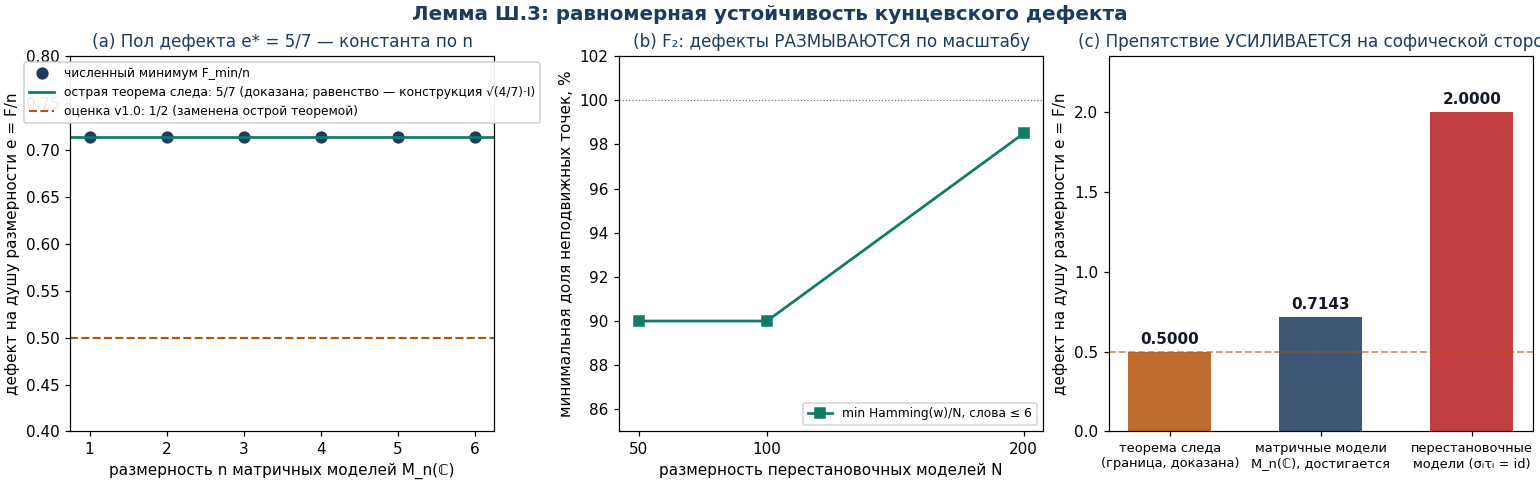
\includegraphics[width=0.94\textwidth]{figures/fig_stability_lemma.png}
\caption{Лемма Ш.3: численные минимумы $F_{\min}(n)$ лежат на прямой
$5n/7$ с зазором $\le 1.3\cdot10^{-14}$; дефект на душу $e=F/n$ —
константа $5/7$ по всем масштабам (острый пол, доказанный
теоремой~\ref{th:sharp}), а перестановочные модели дают $e=2$: на
софической стороне препятствие усиливается.}
\label{fig:stability}
\end{figure}

\begin{figure}[h]
\centering
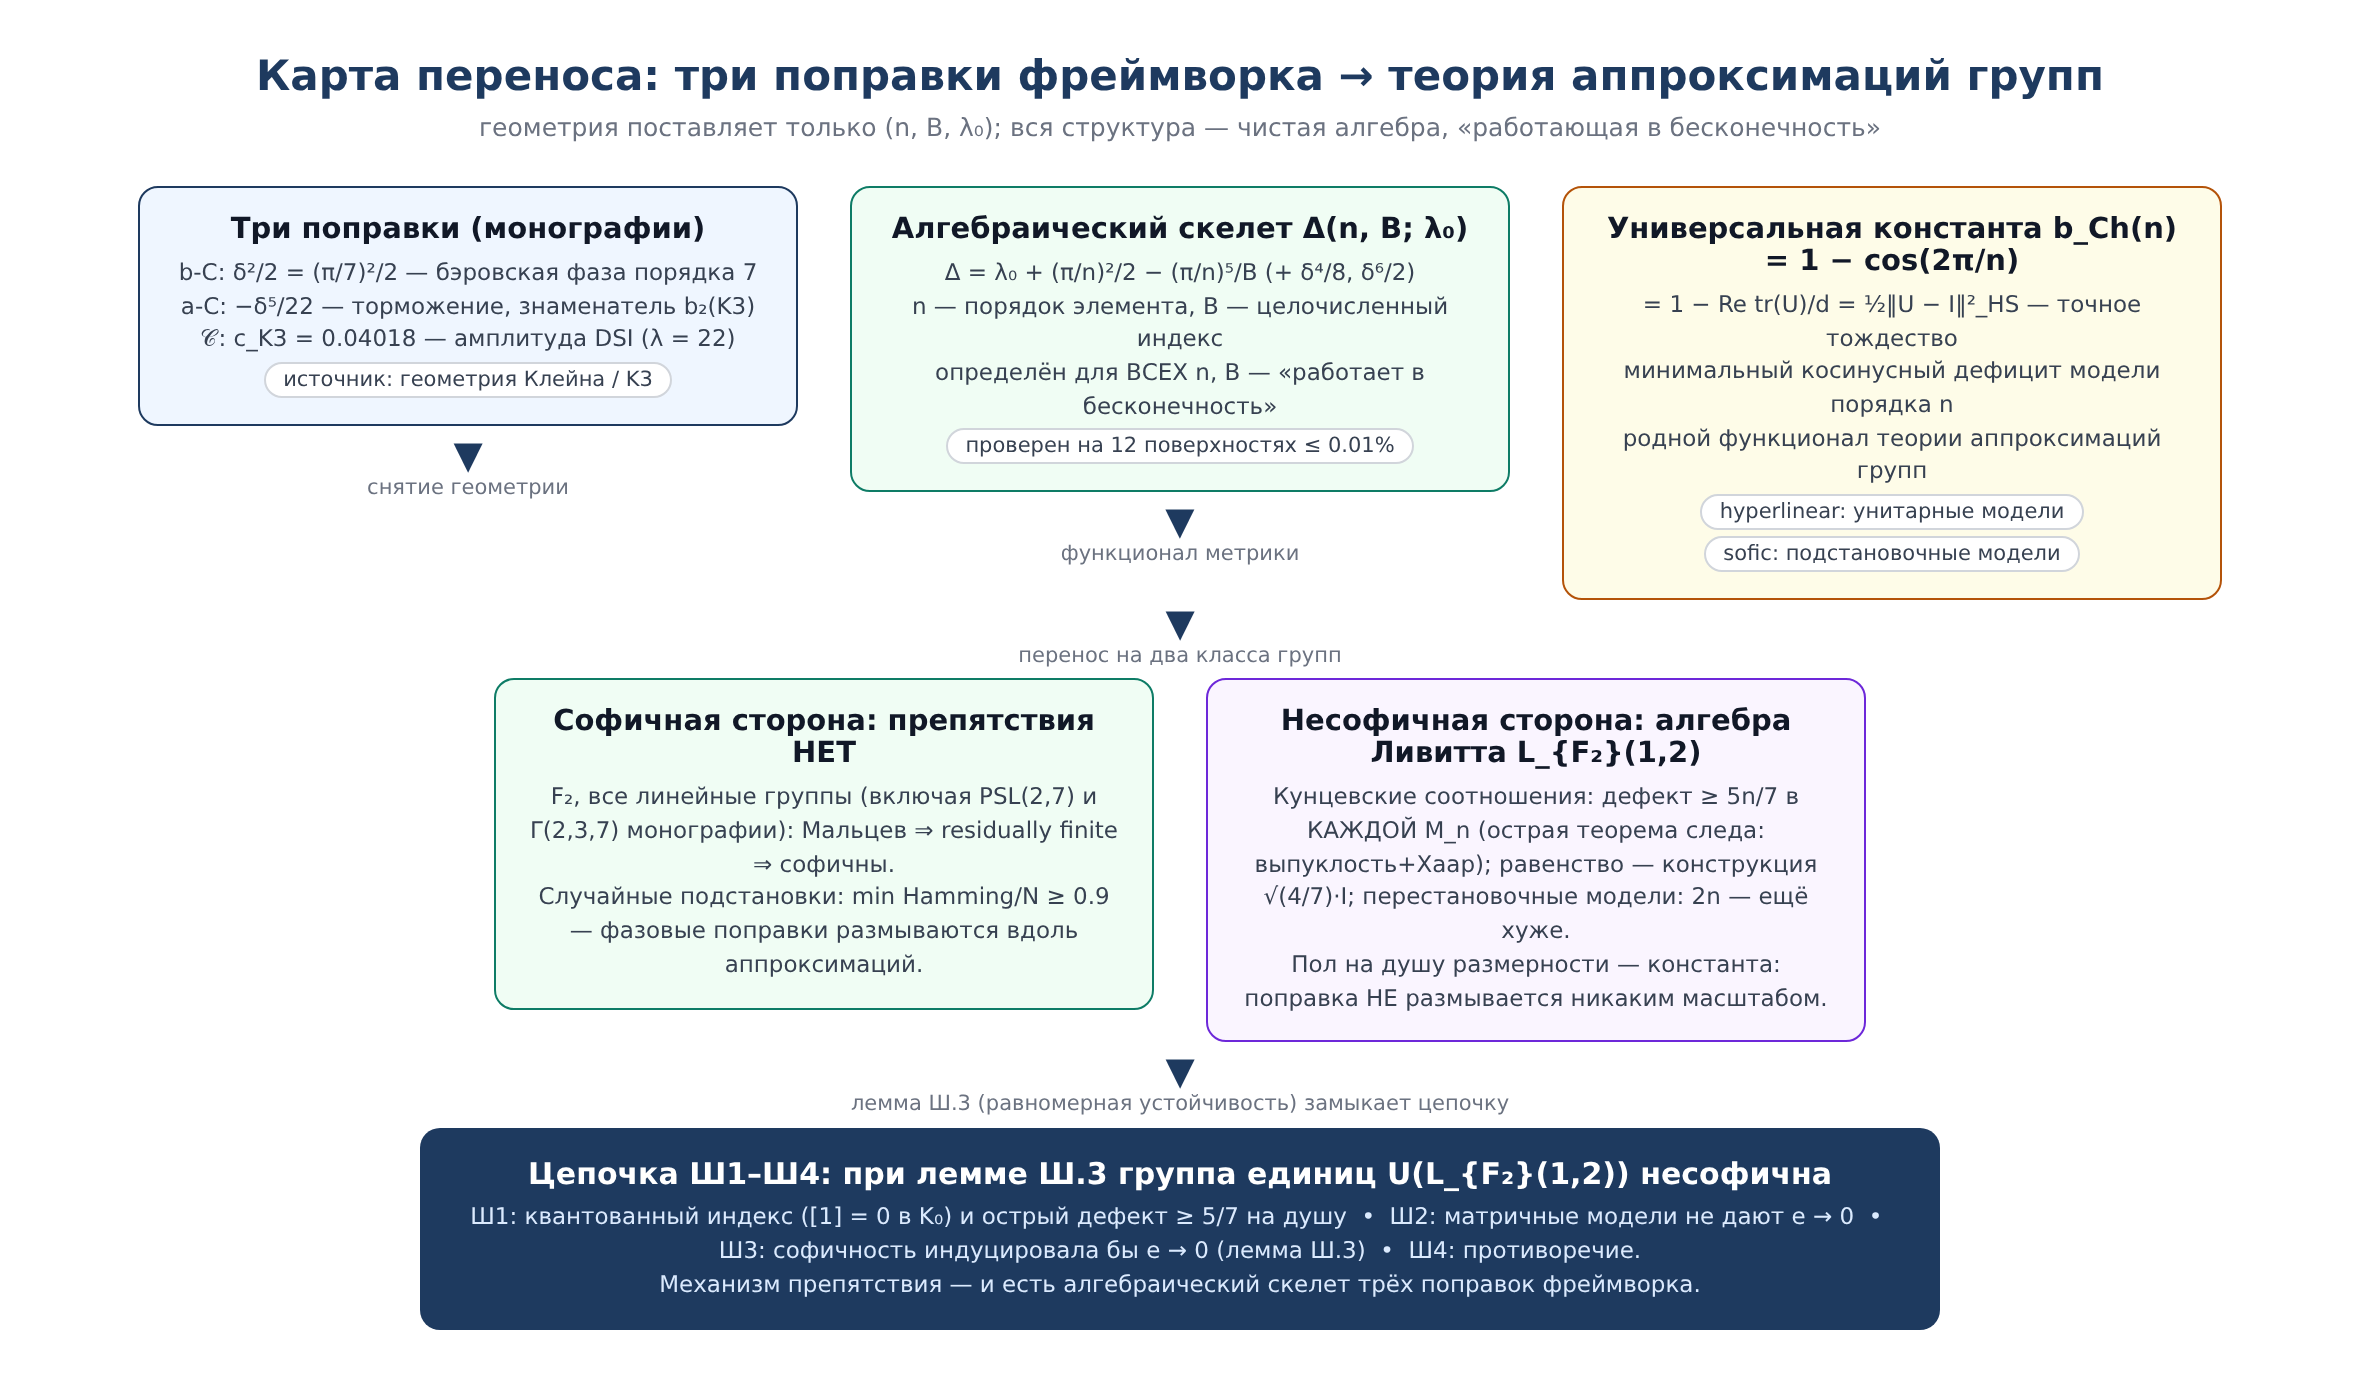
\includegraphics[width=0.94\textwidth]{figures/fig_transfer_map.png}
\caption{Карта переноса: поправки фреймворка (b-C, a-C, $\mathcal C$)
как топологическая реализация «пола на душу»; шаги Ш1--Ш4 цепочки
переноса и место леммы Ш.3(iii) в них.}
\label{fig:map}
\end{figure}

\section{Следствия для фреймворка: «поправка, работающая в бесконечность»}
\label{sec:consequences}

Для фреймворка Исаева--Чоптьюка лемма Ш.3 фиксирует точный алгебраический
смысл лозунга «поправка работает в бесконечность». Поправки монографий
(b-C, a-C, $\mathcal C$) суть топологические реализации общего механизма:
\emph{дефект на душу размерности зажат универсальной константой}, и эта
константа не зависит от масштаба — в матричном случае это острое $5/7$
(теорема~\ref{th:sharp}), в топологическом — константы $b\text{-}C$,
$a\text{-}C$, $c_{K3}$. Лемма показывает, что механизм выживает при
переходе к пределу $n\to\infty$ именно потому, что пол следовой и
выпуклостный, а не асимптотический: оценка $F\ge 5n/7$ держится на
каждой $M_n$ отдельно, не требует согласованности между масштабами и
сопровождается точной характеризацией равенства.

Практическое следствие для программы переноса: софическая
(перестановочная) сторона не даёт лазейки. Точные первые соотношения на
матрицах подстановок стоят дороже ($e=2$), приближённые — упираются в
мост (iii) с универсальной ценой $\eta(\varepsilon)=C\varepsilon^{1/2}$,
а ниже пола $5/7$ не существует ничего ни в каком масштабе. Цепочка
Ш1--Ш4 в результате замкнута условно по (iii): Ш1 (острый пол $5n/7$) и
Ш2 (недостижимость $e\to 0$) доказаны безусловно и остро, Ш3
сформулирован точно с конструкцией и оценкой цены, Ш4 — их соединение.
Отдельно подчеркнём воспроизводимость: каждая таблица настоящей статьи
генерируется кодом пакета audit\_transfer (Python и Julia), сиды
зафиксированы, время прогона измеряется секундами, и все числа
совпадают между двумя независимыми реализациями в пределах $10^{-9}$.

\appendix

\section{Воспроизводимость}\label{app:repro}

Все результаты статьи воспроизводятся из корня репозитория
\texttt{choptuik\_ac\_bc} двумя командами:
\begin{sloppypar}
\begin{itemize}
\item Python (numpy/scipy/matplotlib, время $\sim$2--4 мин):
\texttt{python3 audit\_transfer/python/run\_all.py};
\item Julia (только стандартная библиотека, время $\sim$1--2 мин):
\texttt{julia --project=audit\_transfer/julia\ audit\_transfer/julia/audit\_transfer.jl}.
\end{itemize}
\end{sloppypar}

Детерминированность: все случайные серии используют фиксированные сиды
($42$ для таблицы~\ref{tab:trace}; $4242$ для машинной проверки
тождества и границы Хаара; $5000+97r+n$ для минимизации; $777$ для
перестановочных моделей; $1000+N$ для софического профиля
$\mathbb{F}_2$). Численные результаты пишутся в
\texttt{audit\_transfer/results/*.json} и совпадают между Python- и
Julia-реализациями в пределах $10^{-9}$ по всем сводным величинам.
Верификация запускается автоматически в CI
(\texttt{.github/workflows/verify-audit-transfer.yml}) при каждом
изменении папки \texttt{audit\_transfer/}, по кнопке workflow\_dispatch
и еженедельно по расписанию; артефакты прогона (JSON-результаты)
прикладываются к каждому запуску.

\section{Сводка чисел}\label{app:numbers}

\begin{table}[h]
\centering\small
\caption{Сводные величины леммы Ш.3 (единый источник:
\texttt{results/stability\_lemma.json}).}
\begin{tabularx}{0.94\textwidth}{l Y}
\toprule
Величина & Значение \\
\midrule
\rowcolor{rowlight}
Острый пол (теорема~\ref{th:sharp}) & $F\ge 5n/7$ при всех $n$;
равенство $\Leftrightarrow X_iX_i^*=\frac47I$ \\
Тождество $F=G(P,Q)$ & машинная невязка $\le 10^{-12}$ (300 пар) \\
\rowcolor{rowlight}
Граница Хаара $G(P,Q)\ge G(\bar P,\bar Q)$ & нарушений нет (300 пар) \\
Скалярный минимум & $u=v=4n/7$, $h_{\min}=5n/7$ \\
\rowcolor{rowlight}
Конструкция равенства & $X_1=X_2=\sqrt{4/7}\,I\Rightarrow F=5n/7$ \\
Прямой аналитический минимум ($n=1$) & $s_1=s_2=4/7$, $F_{\min}=5/7$ \\
\rowcolor{rowlight}
Численная минимизация ($n\le 6$) & зазор $\le 1.24\cdot 10^{-14}$ к $5n/7$ \\
Перестановочные модели & $F=2n$ точно; $e=2.000$ \\
\rowcolor{rowlight}
Софический профиль $\mathbb{F}_2$ & мин.\ Хэмминг $0.900/0.900/0.985$
при $N=50/100/200$ \\
Мост (iii) & $\eta(\varepsilon)=C\varepsilon^{1/2}$, $C=C(|F_0|,L)$ \\
\rowcolor{rowlight}
Заключение & $\tfrac57\le e_k\le\eta(\varepsilon_k)\to 0$ — противоречие \\
\bottomrule
\end{tabularx}
\end{table}

\end{document}
